\documentclass{article}

% chinese fonts
\usepackage{ctex}

% math fonts
\usepackage{amsmath}
\usepackage{amsthm}
\usepackage{amssymb}
\usepackage{bm}

% figures
\usepackage{tikz}
\usepackage{graphicx}
\graphicspath{{./figures/}}

% tables
\usepackage{tabularx}
\usepackage{booktabs}
\usepackage{multirow}

% codes
\usepackage{listings}
\lstset{language     = Matlab,
        basicstyle   = \ttfamily,
        keywordstyle = \color{cyan},
        rulecolor    = \color{black},
        commentstyle = \color{green},
        keepspaces   = true,
        tabsize      = 4,
}

% hyperlinks
\usepackage{hyperref}
\hypersetup{
  breaklinks,
  colorlinks = true,
  citecolor  = blue,
  linkcolor  = red,
  urlcolor   = magenta,
}

% algorithms
\usepackage{algorithm}
\usepackage{algorithmic}

% bibliography
\usepackage[sort&compress,numbers]{natbib}

% About:  Macros for Vector, Matrix, Tensor, Math Operator and Misc
% Author: Jingxuan Yang

% vectors
\newcommand{\va}{\bm{a}}       \newcommand{\vah}{\hat{\bm{a}}}        \newcommand{\ah}{\hat{a}}    \newcommand{\vat}{\tilde{\bm{a}}}       \newcommand{\at}{\tilde{a}}
\newcommand{\vb}{\bm{b}}       \newcommand{\vbh}{\hat{\bm{b}}}        \newcommand{\bh}{\hat{b}}    \newcommand{\vbt}{\tilde{\bm{b}}}       \newcommand{\bt}{\tilde{b}}
\newcommand{\vc}{\bm{c}}       \newcommand{\vch}{\hat{\bm{c}}}        \newcommand{\ch}{\hat{c}}    \newcommand{\vct}{\tilde{\bm{c}}}       \newcommand{\ct}{\tilde{c}}
\newcommand{\vd}{\bm{d}}       \newcommand{\vdh}{\hat{\bm{d}}}        \newcommand{\dhat}{\hat{d}}  \newcommand{\vdt}{\tilde{\bm{d}}}       \newcommand{\dt}{\tilde{d}}
\newcommand{\ve}{\bm{e}}       \newcommand{\veh}{\hat{\bm{e}}}        \newcommand{\eh}{\hat{e}}    \newcommand{\vet}{\tilde{\bm{e}}}       \newcommand{\et}{\tilde{e}}
\newcommand{\vf}{\bm{f}}       \newcommand{\vfh}{\hat{\bm{f}}}        \newcommand{\fh}{\hat{f}}    \newcommand{\vft}{\tilde{\bm{f}}}       \newcommand{\ft}{\tilde{f}}
\newcommand{\vg}{\bm{g}}       \newcommand{\vgh}{\hat{\bm{g}}}        \newcommand{\gh}{\hat{g}}    \newcommand{\vgt}{\tilde{\bm{g}}}       \newcommand{\gt}{\tilde{g}}
\newcommand{\vh}{\bm{h}}     \newcommand{\vhh}{\hat{\bm{h}}}        \newcommand{\hh}{\hat{h}}    \newcommand{\vht}{\tilde{\bm{h}}}       \newcommand{\htild}{\tilde{h}}
\newcommand{\vi}{\bm{i}}       \newcommand{\vih}{\hat{\bm{i}}}        \newcommand{\ih}{\hat{i}}    \newcommand{\vit}{\tilde{\bm{i}}}       \newcommand{\itild}{\tilde{i}}
\newcommand{\vj}{\bm{j}}       \newcommand{\vjh}{\hat{\bm{j}}}        \newcommand{\jh}{\hat{j}}    \newcommand{\vjt}{\tilde{\bm{j}}}       \newcommand{\jt}{\tilde{j}}
\newcommand{\vk}{\bm{k}}       \newcommand{\vkh}{\hat{\bm{k}}}        \newcommand{\kh}{\hat{k}}    \newcommand{\vkt}{\tilde{\bm{k}}}       \newcommand{\kt}{\tilde{k}}
\newcommand{\vl}{\bm{l}}       \newcommand{\vlh}{\hat{\bm{l}}}        \newcommand{\lh}{\hat{l}}    \newcommand{\vlt}{\tilde{\bm{l}}}       \newcommand{\lt}{\tilde{l}}
\newcommand{\vm}{\bm{m}}       \newcommand{\vmh}{\hat{\bm{m}}}        \newcommand{\mh}{\hat{m}}    \newcommand{\vmt}{\tilde{\bm{m}}}       \newcommand{\mt}{\tilde{m}}
\newcommand{\vn}{\bm{n}}       \newcommand{\vnh}{\hat{\bm{n}}}        \newcommand{\nh}{\hat{n}}    \newcommand{\vnt}{\tilde{\bm{n}}}       \newcommand{\nt}{\tilde{n}}
\newcommand{\vo}{\bm{o}}       \newcommand{\voh}{\hat{\bm{o}}}        \newcommand{\oh}{\hat{o}}    \newcommand{\vot}{\tilde{\bm{o}}}       \newcommand{\ot}{\tilde{o}}
\newcommand{\vp}{\bm{p}}       \newcommand{\vph}{\hat{\bm{p}}}        \newcommand{\ph}{\hat{p}}    \newcommand{\vpt}{\tilde{\bm{p}}}       \newcommand{\pt}{\tilde{p}}
\newcommand{\vq}{\bm{q}}       \newcommand{\vqh}{\hat{\bm{q}}}        \newcommand{\qh}{\hat{q}}    \newcommand{\vqt}{\tilde{\bm{q}}}       \newcommand{\qt}{\tilde{q}}
\newcommand{\vr}{\bm{r}}       \newcommand{\vrh}{\hat{\bm{r}}}        \newcommand{\rh}{\hat{r}}    \newcommand{\vrt}{\tilde{\bm{r}}}       \newcommand{\rt}{\tilde{r}}
\newcommand{\vs}{\bm{s}}       \newcommand{\vsh}{\hat{\bm{s}}}        \newcommand{\sh}{\hat{s}}    \newcommand{\vst}{\tilde{\bm{s}}}       \newcommand{\st}{\tilde{s}}
\newcommand{\vt}{\bm{t}}       \newcommand{\vth}{\hat{\bm{t}}}        \newcommand{\that}{\hat{t}}  \newcommand{\vtt}{\tilde{\bm{t}}}       \newcommand{\ttil}{\tilde{t}}
\newcommand{\vu}{\bm{u}}       \newcommand{\vuh}{\hat{\bm{u}}}        \newcommand{\uh}{\hat{u}}    \newcommand{\vut}{\tilde{\bm{u}}}       \newcommand{\ut}{\tilde{u}}
\newcommand{\vv}{\bm{v}}       \newcommand{\vvh}{\hat{\bm{v}}}        \newcommand{\vhat}{\hat{v}}    \newcommand{\vvt}{\tilde{\bm{v}}}       \newcommand{\vtild}{\tilde{v}}
\newcommand{\vw}{\bm{w}}       \newcommand{\vwh}{\hat{\bm{w}}}        \newcommand{\wh}{\hat{w}}    \newcommand{\vwt}{\tilde{\bm{w}}}       \newcommand{\wt}{\tilde{w}}
\newcommand{\vx}{\bm{x}}       \newcommand{\vxh}{\hat{\bm{x}}}        \newcommand{\xh}{\hat{x}}    \newcommand{\vxt}{\tilde{\bm{x}}}       \newcommand{\xt}{\tilde{x}}
\newcommand{\vy}{\bm{y}}       \newcommand{\vyh}{\hat{\bm{y}}}        \newcommand{\yh}{\hat{y}}    \newcommand{\vyt}{\tilde{\bm{y}}}       \newcommand{\yt}{\tilde{y}}
\newcommand{\vz}{\bm{z}}       \newcommand{\vzh}{\hat{\bm{z}}}        \newcommand{\zh}{\hat{z}}    \newcommand{\vzt}{\tilde{\bm{z}}}       \newcommand{\zt}{\tilde{z}}

\newcommand{\valpha}{\bm{\alpha}}
\newcommand{\vbeta}{\bm{\beta}}
\newcommand{\vgamma}{\bm{\gamma}}
\newcommand{\vtheta}{\bm{\theta}}
\newcommand{\vlambda}{\bm{\lambda}}
\newcommand{\vmu}{\bm{\mu}}
\newcommand{\vomega}{\bm{\omega}}

\newcommand{\mSigma}{\bm{\Sigma}}

\newcommand{\Fc}{\mathcal{F}}
\newcommand{\Xc}{\mathcal{X}}
\newcommand{\Yc}{\mathcal{Y}}
\newcommand{\Zc}{\mathcal{Z}}
\newcommand{\Gc}{\mathcal{G}}
\newcommand{\Hc}{\mathcal{H}}
\newcommand{\Dc}{\mathcal{D}}
\newcommand{\Cc}{\mathcal{C}}
\newcommand{\Rc}{\mathcal{R}}

% matrices
\newcommand{\ma}{\bm{A}}
\newcommand{\mb}{\bm{B}}
\newcommand{\md}{\bm{D}}
\newcommand{\mH}{\bm{H}}
\newcommand{\mE}{\bm{E}}
\newcommand{\mi}{\bm{I}}
\newcommand{\mk}{\bm{K}}
\newcommand{\ml}{\bm{L}}
\newcommand{\mn}{\bm{N}}
\newcommand{\mP}{\bm{P}}
\newcommand{\mq}{\bm{Q}}
\newcommand{\mr}{\bm{R}}
\newcommand{\mU}{\bm{u}}
\newcommand{\mv}{\bm{v}}
\newcommand{\mw}{\bm{W}}
\newcommand{\mx}{\bm{X}}
\newcommand{\my}{\bm{Y}}
\newcommand{\mz}{\bm{Z}}

% tensors
\newcommand{\tp}{\mathsf{P}}
\newcommand{\tu}{\mathsf{U}}
\newcommand{\tx}{\mathsf{X}}
\newcommand{\ty}{\mathsf{Y}}
\newcommand{\tz}{\mathsf{Z}}
\newcommand{\tw}{\mathsf{W}}
\newcommand{\tf}{\mathsf{F}}
\newcommand{\ta}{\mathsf{A}}
\renewcommand{\th}{\mathsf{H}}

% norms
\newcommand{\mynorm}[2]{\| {#1} \|_{#2}}
\newcommand{\norm}[2]{\mynorm{#1}{#2}}
\newcommand{\bignorm}[2]{\left\| {#1} \right\|_{#2}}
\newcommand{\norml}[1]{\mynorm{#1}{1}}
\newcommand{\bignorml}[1]{\bignorm{#1}{1}}
\newcommand{\infnorm}[1]{\mynorm{#1}{\infty}}
\newcommand{\biginfnorm}[1]{\bignorm{#1}{\infty}}
\newcommand{\oneinf}{\ell_{1,\infty}}
\newcommand{\onetwo}{\ell_{1,2}}
\newcommand{\oneinfnorm}[1]{\mynorm{#1}{1,\infty}}
\newcommand{\bigoneinf}[1]{\bignorm{#1}{1,\infty}}
\newcommand{\onetwonorm}[1]{\mynorm{#1}{1,2}}
\newcommand{\bigonetwo}[1]{\bignorm{#1}{1,2}}
\newcommand{\enorm}[1]{\mynorm{#1}{2}}
\newcommand{\bigenorm}[1]{\bignorm{#1}{2}}
\newcommand{\znorm}[1]{\mynorm{#1}{0}}
\newcommand{\bigznorm}[1]{\bignorm{#1}{0}}
\newcommand{\frob}[1]{\|{#1}\|_{\text{F}}}
\newcommand{\bigfrob}[1]{\bignorm{#1}{\text{F}}}
\newcommand{\grpnorm}[2]{\norm{#1}{\text{Gr}(#2)}}

% math operators
\DeclareMathOperator*{\argmin}{argmin}
\DeclareMathOperator*{\argmax}{argmax}
\DeclareMathOperator{\divg}{div}
\DeclareMathOperator{\dom}{dom}
\DeclareMathOperator{\interior}{int}
\DeclareMathOperator{\ri}{ri}
\DeclareMathOperator{\sgn}{sgn}
\DeclareMathOperator{\trace}{Tr}
\DeclareMathOperator{\diag}{diag}
\DeclareMathOperator{\rank}{rank}
\DeclareMathOperator{\range}{range}
\DeclareMathOperator{\vect}{vec}
\DeclareMathOperator{\prox}{prox}
\DeclareMathOperator{\intr}{int}
\DeclareMathOperator{\relint}{ri}

% misc
\newcommand{\gs}{\geqslant}
\newcommand{\ls}{\leqslant}
\newcommand{\set}[1]{\left\{ {#1}\right\}}

\newcommand{\defeq}{\ \stackrel{\text{def}}{=}\ }
\newcommand{\ip}[2]{\left\langle#1, #2\right\rangle}
\newcommand{\reals}{\mathbb{R}}
\newcommand{\complex}{\mathbb{C}}
\newcommand{\half}{\frac{1}{2}}

\newtheorem{theorem}{Theorem}
\newtheorem{lemma}[theorem]{Lemma}
\newtheorem{proposition}[theorem]{Proposition}
\newtheorem{remark}[theorem]{Remark}
\newtheorem{corollary}[theorem]{Corollary}
\newtheorem{definition}[theorem]{Definition}


\setlength{\oddsidemargin}{-0.25 in}
\setlength{\evensidemargin}{-0.25 in} 
\setlength{\topmargin}{-0.25in} 
\setlength{\textwidth}{7 in} 
\setlength{\textheight}{8.5 in}
\setlength{\headsep}{0.25 in} 
\setlength{\parindent}{0 in}
\setlength{\parskip}{0.1 in}

\newcommand{\homework}[5]{
  \pagestyle{myheadings} 
  \thispagestyle{plain}
  \newpage
  \setcounter{page}{1} 
  \setcounter{section}{#5} 
  \noindent
  \begin{center}
    \framebox{ 
      \vbox{
        \vspace{2mm} 
        \hbox to 6.28in { {\bf
        THU-70250043-0,~Pattern~Recognition~(Spring 2021) \hfill Homework: 6} }
        \vspace{6mm} 
        \hbox to 6.28in { {\Large \hfill #1 \hfill} }
        \vspace{6mm} 
        \hbox to 6.28in { {\it Lecturer: #2 \hfill} }
        \vspace{2mm} 
        \hbox to 6.28in { {\it \hspace{14mm} #3 \hfill} }
        \vspace{2mm} 
        \hbox to 6.28in { {\it Student: #4 \hfill} }
        \vspace{2mm} 
      } 
    }
  \end{center}
  \markboth{#1}{#1} 
  \vspace*{4mm} 
}

\begin{document}

\homework{$k$-NN and Metric}{Changshui Zhang
\hspace{5mm} {\tt zcs@mail.tsinghua.edu.cn}}{Hong Zhao \hspace{16mm} {\tt vzhao@tsinghua.edu.cn}}{Jingxuan Yang \hspace{10mm} {\tt yangjx20@mails.tsinghua.edu.cn}}{8}

\section*{Property of Euclidean Distance}

1. When the metric space is a finite-dimensional Euclidean space, please prove that the Voronoi cells induced by the single-nearest neighbor algorithm must always be convex. Does this property hold when the metric becomes Manhattan distance?

In mathematics, a Voronoi diagram is a partition of a plane into regions close to each of a given set of objects. In the simplest case, these objects are just finitely many points in the plane (called seeds, sites, or generators). For each seed there is a corresponding region consisting of all points of the plane closer to that seed than to any other. These regions are called Voronoi cells, as shown in Figure~\ref{pic1}. Similarly, Voronoi cells of a discrete set in higher-order Euclidean space are known as generalized polyhedra.

\begin{figure}[ht]
	\centering
	
\includegraphics[scale=0.3]{Euclidean_Voronoi_diagram.pdf}
	\caption{Voronoi cells with Euclidean distance \cite{pics}.}
	\label{pic1}
\end{figure}

\emph{Hint}: Convex means for any two points $x_1$ and $x_2$ in a cell, all points on the segment linking $x_1$ and $x_2$ must also lie in the cell.

证明: 令 $\{x_1,x_2,\dots,x_n\}$ 为 $n$ 个样本点, $V_i$, $i=1,2,\dots,n$ 表示 $x_i$ 所在的由 $\ell_2$ 范数 (Euclidean Distance) 最近邻法生成的 Voronoi 区域. 设 $\xi_1,~\xi_2\in V_i$, 即有
\begin{equation}
  \begin{aligned}
    \|\xi_1-x_i\|&\ls\|\xi_1-x_j\|,~\forall~j\neq i\\
    \|\xi_2-x_i\|&\ls\|\xi_2-x_j\|,~\forall~j\neq i\\
  \end{aligned}
\end{equation}

对 $\xi=\lambda\xi_1+(1-\lambda)\xi_2$, $0\ls\lambda\ls1$, $\forall~j\neq i$, 由上式及余弦定理
\begin{equation}
  \langle a,b\rangle = a^\top b = \frac{\|a\|^2+\|b\|^2-\|a-b\|^2}{2}
\end{equation}

可得
\begin{equation}
  \begin{aligned}
    \|\xi-x_i\|^2
    &=\|\lambda\xi_1+(1-\lambda)\xi_2-x_i\|^2\\
    &=\|\lambda(\xi_1-x_i)+(1-\lambda)(\xi_2-x_i)\|^2\\
    &=\lambda^2\|\xi_1-x_i\|^2+2\lambda(1-\lambda)(\xi_1-x_i)^\top(\xi_2-x_i)+(1-\lambda)^2\|(\xi_2-x_i)\|^2\\
    &=\lambda^2\|\xi_1-x_i\|^2+\lambda(1-\lambda)(\|\xi_1-x_i\|^2+\|\xi_2-x_i\|^2-\|\xi_1-\xi_2\|^2)+(1-\lambda)^2\|(\xi_2-x_i)\|^2\\
    &=\lambda\|\xi_1-x_i\|^2-\lambda(1-\lambda)\|\xi_1-\xi_2\|^2+(1-\lambda)\|(\xi_2-x_i)\|^2\\
    &\ls\lambda\|\xi_1-x_j\|^2-\lambda(1-\lambda)\|\xi_1-\xi_2\|^2+(1-\lambda)\|\xi_2-x_j\|^2\\
    &=\|\xi-x_j\|^2
  \end{aligned}
\end{equation}

即
\begin{equation}
  \|\xi-x_i\|\ls\|\xi-x_j\|,~\forall~j\neq i
\end{equation}

因此, $\xi\in V_i$, 即由 $\ell_2$ 范数最近邻法生成的 Voronoi 区域都是凸的. 

由 $\ell_1$ 范数 (Manhattan Distance) 最近邻法生成的 Voronoi 区域不是凸的, 如图 \ref{fig:l1} 所示.

\begin{figure}[ht]
	\centering
	
\includegraphics[width=5.5cm]{Manhattan_Voronoi_Diagram.png}
	\caption{Voronoi cells with Manhattan distance \cite{ManhattanVoronoi}.}
	\label{fig:l1}
\end{figure}

\section*{Properties of Metric}

2. Please prove that the Minkowski metric indeed possesses the three properties required of all metrics.

\emph{Hint}: A metric $D(\cdot,\cdot)$ must have three properties: for all vectors $a$, $b$ and $c$,
\begin{enumerate}
  \item[(1)] Identity of indiscernibles: $D(a, b) = 0$ if and only if $a = b$.
  \item[(2)] Symmetry: $D(a, b) = D(b, a)$.
  \item[(3)] Triangle inequality: $D(a, b) + D(b, c) \gs D(a, c)$.
\end{enumerate}

证明: $s$ ($s\gs1$) 阶 Minkowski 距离为
\begin{equation}
  D(x,y)=\left(\sum_{j=1}^d|x_j-y_j|^s\right)^{1/s}
\end{equation}

首先证明 identity of indiscernibles, $\forall~x,y$, 当 $x=y$ 时, 有
\begin{equation}
  D(x,y)=D(x,x)=\left(\sum_{j=1}^d|x_j-x_j|^s\right)^{1/s}=0
\end{equation}

当 $D(x,y)=0$ 时, 有
\begin{equation}
  \sum_{j=1}^d|x_j-y_j|^s=0
\end{equation}

由于每一项绝对值均非负, 则
\begin{equation}
  x_j=y_j,\quad\forall~j=1,2,\dots,d
\end{equation}

即 $x=y$.

其次证明对称性, $\forall~x,y$, 有
\begin{equation}
  D(x,y)=\left(\sum_{j=1}^d|x_j-y_j|^s\right)^{1/s}=\left(\sum_{j=1}^d|y_j-x_j|^s\right)^{1/s}=D(y,x)
\end{equation}

下面证明三角不等式, $\forall~x,y,z$, 由绝对值性质有
\begin{equation}
  \begin{aligned}
    D(x,y)
    &=\left(\sum_{j=1}^d|x_j-y_j|^s\right)^{1/s}\\
    &=\left(\sum_{j=1}^d|x_j-z_j+z_j-y_j|^s\right)^{1/s}\\
    &\ls\left(\sum_{j=1}^d(|x_j-z_j|+|z_j-y_j|)^s\right)^{1/s}\\
  \end{aligned}
\end{equation}

其中, 由 H{\"o}lder 不等式可得
\begin{equation}
  \begin{aligned}
    \sum_{j=1}^d(|x_j-z_j|+|z_j-y_j|)^s
    &=\sum_{j=1}^d(|x_j-z_j|+|z_j-y_j|)\cdot(|x_j-z_j|+|z_j-y_j|)^{s-1}\\
    &=\sum_{j=1}^d(|x_j-z_j|+|z_j-y_j|)\cdot(|x_j-z_j|+|z_j-y_j|)^{s/t},\quad \frac{1}{s}+\frac{1}{t}=1\\
    &=\sum_{j=1}^d|x_j-z_j|\cdot(|x_j-z_j|+|z_j-y_j|)^{s/t}+\sum_{j=1}^d|z_j-y_j|\cdot(|x_j-z_j|+|z_j-y_j|)^{s/t}\\
    &\ls\left[\left(\sum_{j=1}^d|x_j-z_j|^s\right)^{1/s}+\left(\sum_{j=1}^d|z_j-y_j|^s\right)^{1/s}\right]\left(\sum_{j=1}^d(|x_j-z_j|+|z_j-y_j|)^{s}\right)^{1/t}\\
  \end{aligned}
\end{equation}

整理即得
\begin{equation}
    \left(\sum_{j=1}^d(|x_j-z_j|+|z_j-y_j|)^s\right)^{1-1/t}
    \ls\left(\sum_{j=1}^d|x_j-z_j|^s\right)^{1/s}+\left(\sum_{j=1}^d|z_j-y_j|^s\right)^{1/s}
\end{equation}

又 $1-\frac{1}{t}=\frac{1}{s}$, 则
\begin{equation}
  \left(\sum_{j=1}^d(|x_j-z_j|+|z_j-y_j|)^s\right)^{1/s}
  \ls\left(\sum_{j=1}^d|x_j-z_j|^s\right)^{1/s}+\left(\sum_{j=1}^d|z_j-y_j|^s\right)^{1/s}
\end{equation}

此即 Minkowski 不等式, 所以
\begin{equation}
  \begin{aligned}
    D(x,y)
    &\ls\left(\sum_{j=1}^d(|x_j-z_j|+|z_j-y_j|)^s\right)^{1/s}\\
    &\ls\left(\sum_{j=1}^d|x_j-z_j|^s\right)^{1/s}+\left(\sum_{j=1}^d|z_j-y_j|^s\right)^{1/s}\\
    &=D(x,z)+D(z,y)
  \end{aligned}
\end{equation}

因此, 三角不等式成立.\qed

本题用到的 H{\"o}lder 不等式可由 Jensen 不等式证明如下 \cite{Holder_inequality}. 简便起见, 对向量 $\va=(a_1,a_2,\dots,a_n)\in\reals^n$ 和 $p\gs1$, 定义 $\ell_p$ 范数为
\begin{equation}
  \|\va\|_p=\left(\sum_{k=1}^n|a_k|^p\right)^{1/p},
\end{equation}

则 H{\"o}lder 不等式可表述为对 $p\gs1$ 和 $\forall~\va,\vb\in\reals_+^n$, 有
\begin{equation}
  \sum_{k=1}^na_kb_k\ls\|\va\|_p~\|\vb\|_q,\quad\frac{1}{p}+\frac{1}{q}=1.
\end{equation}

证明: 对凸函数 $f(x)=x^p$ 应用 Jensen 不等式有
\begin{equation}
  \left(\sum_{k=1}^n\lambda_kx_k\right)^p\ls\sum_{k=1}^n\lambda_kx_k^p,\quad\sum_{k=1}^n\lambda_k=1,~\lambda_k\gs0,~k=1,2,\dots,n
\end{equation}

取 $a_k=\lambda_k^{1/p}x_k$, $c_k=\lambda_k^{1/q}$, 则上式变为
\begin{equation}
  \sum_{k=1}^na_kc_k\ls\left(\sum_{k=1}^na_k^p\right)^{1/p},\quad\sum_{k=1}^nc_k^q=1,~c_k\gs0,~k=1,2,\dots,n
\end{equation}

取
\begin{equation}
  c_k=\frac{b_k}{\|\vb\|_q}
\end{equation}

满足
\begin{equation}
  \sum_{k=1}^nc_k^q=1,~c_k\gs0,~k=1,2,\dots,n
\end{equation}

则有
\begin{equation}
  \sum_{k=1}^na_k\frac{b_k}{\|\vb\|_q}\ls\left(\sum_{k=1}^na_k^p\right)^{1/p}=\|\va\|_p
\end{equation}

即
\begin{equation}
  \sum_{k=1}^na_kb_k\ls\|\va\|_p~\|\vb\|_q
\end{equation}

因此, H{\"o}lder 不等式成立.\qed

\section*{$k$-NN Classifier}

3. Let $\mathcal{D}=\{\vx_1,\vx_2,\dots,\vx_n\}$ be a set of $n$ independent labelled samples and let $\mathcal{D}_k(\vx)=\{\vx'_1,\vx'_2,\dots,\vx'_k\}$ be the $k$ nearest neighbors of $\vx$. Recall that the $k$-nearest-neighbor rule for classifying $\vx$ is to give $\vx$ the label most frequently represented in $\mathcal{D}_k(\vx)$. Consider a two-category problem with $P(\omega_1) = P(\omega_2) = 1/2$. Assume further that the conditional densities $p(x|\omega_i)$ are uniform within unit hyperspheres, and the two categories center on two points ten units apart. Figure \ref{pic2} shows a diagram of this situation.
\begin{figure}[ht]
	\centering
	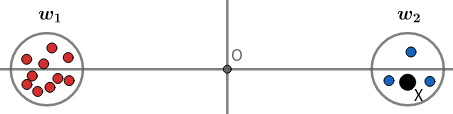
\includegraphics[scale=0.5]{diagram.png}
	\caption{A diagram of assumed situation. When $k\gs7$, X is misclassified as there are only $3$ samples in $\omega_2$.}
	\label{pic2}
\end{figure}

3.1. Show that if $k$ is odd, the average probability of error is given by
\begin{equation}\nonumber
    P_n(e)=\frac{1}{2^n}\sum_{j=0}^{(k-1)/2}\binom{n}{j}.
\end{equation}

解: 令 $P(x\in\omega_i,\omega_j)$, $i,j=1,2$ 表示 $x$ 属于 $\omega_j$ 类, 但是 $k$-NN 算法将其判断为 $\omega_i$ 类. 当 $\omega_j$ 类的样本数量小于 $(k-1)/2$ 时, 就会出现分类错误的情况, 即此时 $i\neq j$.

因此, 错误率为
\begin{equation}
  \begin{aligned}
    P_n(e)
    &=P(x\in\omega_1,\omega_2)+P(x\in\omega_2,\omega_1)\\
    &=P(x\in\omega_1|\omega_2)P(\omega_2)+P(x\in\omega_2|\omega_1)P(\omega_1)\\
    &=\frac{1}{2}\sum_{j=0}^{(k-1)/2}\binom{n}{j}\left(\frac{1}{2}\right)^j\left(\frac{1}{2}\right)^{n-j}+\frac{1}{2}\sum_{j=0}^{(k-1)/2}\binom{n}{j}\left(\frac{1}{2}\right)^j\left(\frac{1}{2}\right)^{n-j}\\
    &=\frac{1}{2^n}\sum_{j=0}^{(k-1)/2}\binom{n}{j}
  \end{aligned}
\end{equation}

3.2. Show that for this case the single-nearest neighbor rule has a lower error rate than the $k$-nearest-neighbor error rate for $k>1$.

解: 当 $k=1$ 时, 由上题可知最近邻法错误率为
\begin{equation}
  \tilde{P}_n(e)=\frac{1}{2^n}
\end{equation}
当 $k>1$ 时
\begin{equation}
  \begin{aligned}
    P_n(e)
    &=\frac{1}{2^n}\sum_{j=0}^{(k-1)/2}\binom{n}{j}\\
    &=\frac{1}{2^n}\sum_{j=1}^{(k-1)/2}\binom{n}{j}+\frac{1}{2^n}\\
    &>\frac{1}{2^n}=\tilde{P}_n(e)
  \end{aligned}
\end{equation}

即最近邻法错误率 $\tilde{P}_n(e)<P_n(e)$.

3.3. If $k$ is odd and is allowed to increase with $n$ but is restricted by $k < a\sqrt{n}$, where $a$ is a positive constant, show that $P_n(e) \to 0$ as $n \to \infty$.

解: 当 $n\to\infty$ 时, 有
\begin{equation}
  \begin{aligned}
    \lim_{n\to\infty}P_n(e)
    &=\lim_{n\to\infty}\frac{1}{2^n}\sum_{j=0}^{(k-1)/2}\binom{n}{j}\\
    &\ls\lim_{n\to\infty}\frac{1}{2^n}\sum_{j=0}^{\lfloor(a\sqrt{n}-1)/2\rfloor}\binom{n}{j}\\
    &=\lim_{n\to\infty}\frac{1}{2^n}\sum_{j=0}^{\lfloor(a\sqrt{n}-1)/2\rfloor}n^j,\quad\binom{n}{j}=\frac{n!}{j!(n-j)!}\sim n^j\\
    &=\lim_{n\to\infty}\frac{n^{(a\sqrt{n}-1)/2}}{2^n}\\
    &=\lim_{n\to\infty}\frac{n^{a\sqrt{n}/2}}{2^n}\\
    &=\lim_{n\to\infty}\frac{\exp(\frac{a}{2}\sqrt{n}\log n)}{\exp(n\log2)}\\
    &=\lim_{n\to\infty}\exp\left(\frac{a}{2}\sqrt{n}\log n-n\log2\right)\\
    &=\lim_{n\to\infty}\exp\left[-n\log2\cdot\left(1-\frac{a\log n}{2\sqrt{n}\log2}\right)\right]\\
    &=\lim_{n\to\infty}\exp\left[-n\log2\cdot\left(1-\frac{an^{-1}}{n^{-1/2}\log2}\right)\right]\\
    &=\lim_{n\to\infty}\exp(-n\log2)\\
    &=0\\
  \end{aligned}
\end{equation}

又 $P_n(e)\gs0$, 因此
\begin{equation}
  \lim_{n\to\infty}P_n(e)=0
\end{equation}

\section*{Programming: $k$-NN Classifier on MNIST}

4. Please implement $k$-NN classifier and run on MNIST \cite{mnist}. You need to follow the official train/test split of MNIST. Compare the performance with the following settings:

\begin{enumerate}
	\item[-] Using 100, 300, 1000, 3000, 10000 training samples.
	\item[-] Using different values of $k$.
	\item[-] Using at least three different distance metrics.
\end{enumerate}

In this assignment, you are \emph{NOT} allowed to use any existing libraries or code snippets that provides $k$-NN algorithm.

解: 首先分析训练样本数量对算法性能的影响, 分别使用 $n=100,~300,~1000,~3000,~10000$ 个训练样本作为训练集, 比较最近邻分类器 ($k=1$) 的性能变化, 计算采用 Minkowski 距离 $p=2$, 即欧氏距离. $k$-NN 算法的准确率和运行时间分别如图 \ref{fig:sampleAccuracy} 和图 \ref{fig:sampleTime} 所示.

由图可知, 算法的正确率随着样本数量增加而增加, 在样本数量增加到一定值后, 正确率的增长速度变慢; 算法的运行时间随着训练样本数量的增加而近乎线性增加.

\begin{figure}[htbp]
  \centering
  \begin{minipage}[t]{0.48\textwidth}
    \centering
    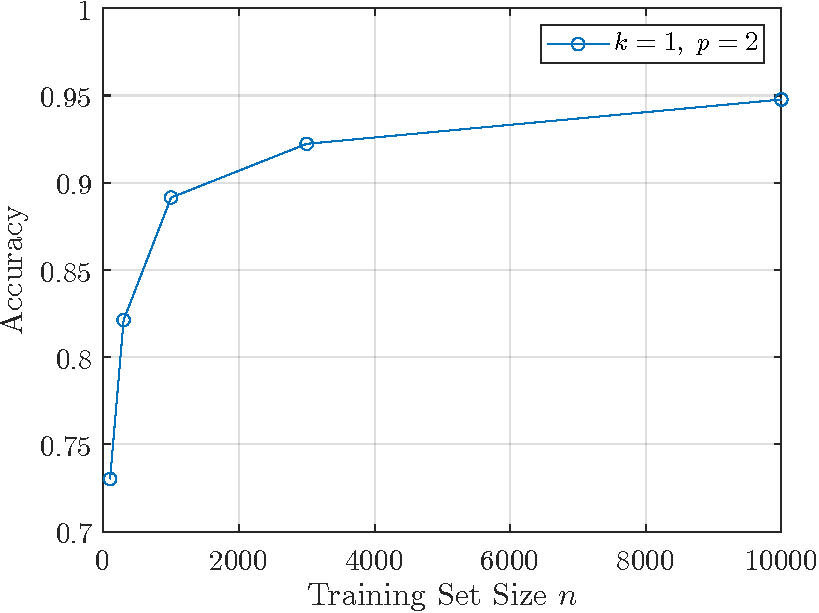
\includegraphics[width=8cm]{sampleAccuracy.pdf}
    \caption{正确率与训练样本数变化关系}
    \label{fig:sampleAccuracy}
  \end{minipage}
  \begin{minipage}[t]{0.48\textwidth}
    \centering
    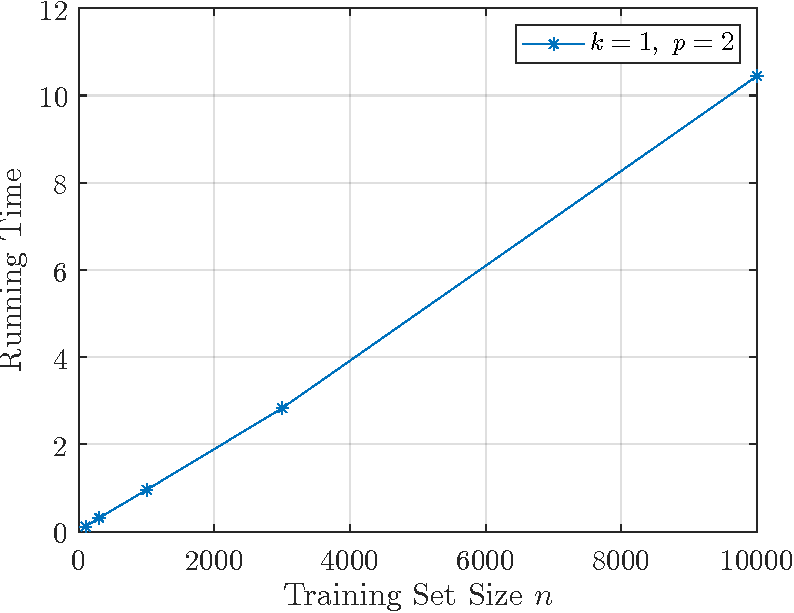
\includegraphics[width=8cm]{sampleTime.pdf}
    \caption{运行时间与训练样本数变化关系}
    \label{fig:sampleTime}
  \end{minipage}
\end{figure}

其次, 分析 $k$-NN 算法的参数 $k$ 对算法性能的影响, 训练样本数取 $n=3000$, Minkowski 距离参数取 $p=2$, 即欧氏距离, 取 $k=[1,100]$, 得到 $k$-NN 算法的准确率和运行时间分别如图 \ref{fig:kAccuracy} 和图 \ref{fig:kTime} 所示.

由图可知, 算法的正确率随着 $k$ 的增加先增加后减小, $k=3$ 时正确率最高, 取过大的 $k$ 反而会使得算法的正确率下降; 算法的运行时间基本稳定在 2.85 s, 与 $k$ 的取值基本无关. 因为 $k$-NN 的时间复杂度主要体现在计算待预测样本点与训练集所有样本点之间的距离, 选择不同的 $k$ 值对实际算法运行时间无明显影响.

\begin{figure}[htbp]
  \centering
  \begin{minipage}[t]{0.48\textwidth}
    \centering
    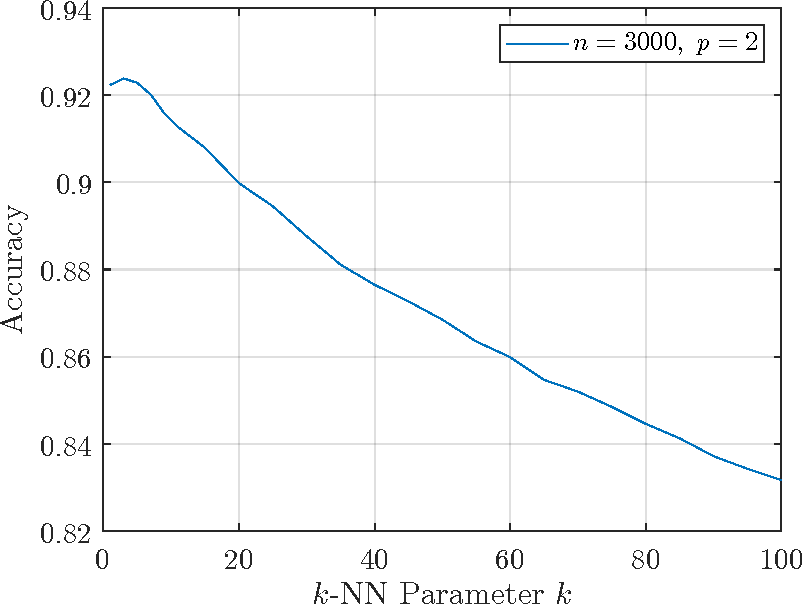
\includegraphics[width=8cm]{kAccuracy.pdf}
    \caption{正确率与 $k$-NN 参数 $k$ 变化关系}
    \label{fig:kAccuracy}
  \end{minipage}
  \begin{minipage}[t]{0.48\textwidth}
    \centering
    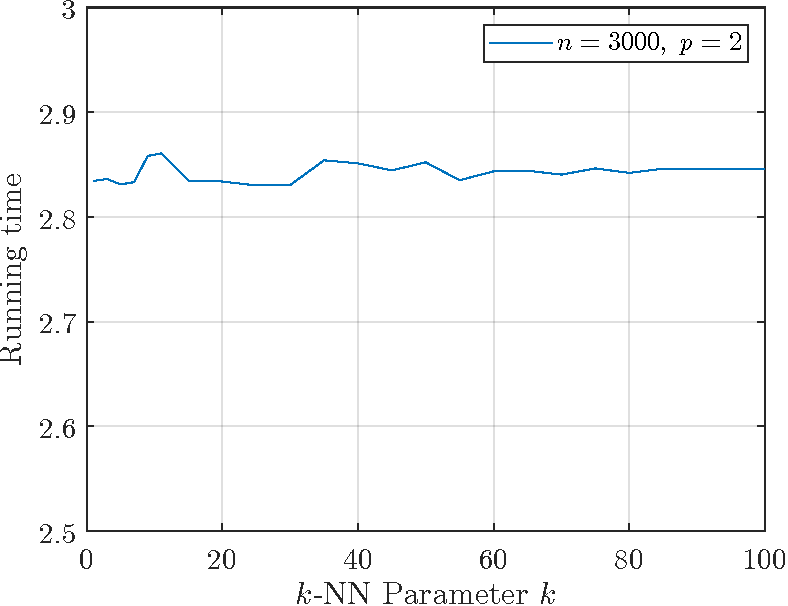
\includegraphics[width=8cm]{kTime.pdf}
    \caption{运行时间与 $k$-NN 参数 $k$ 变化关系}
    \label{fig:kTime}
  \end{minipage}
\end{figure}

最后分析不同的距离对算法性能的影响, 训练样本数取 $n=3000$, 比较最近邻分类器 ($k=1$) 的性能变化, Minkowski 距离参数取 $p=1,~2,~4,~\infty$, 得到 $k$-NN 算法的准确率和运行时间分别如图 \ref{fig:pAccuracy} 和图 \ref{fig:pTime} 所示.

由图可知, 算法的正确率随着 $p$ 的增大而有所增加,但 Chebyshev 距离 ($p=\infty$) 的正确率最低; 算法的运行时间与 $\ell_p$ 范数的计算复杂度有关, $\ell_1,~\ell_2$ 与 $\ell_\infty$ 范数的复杂度基本相同, 而 $\ell_4$ 范数的复杂度远远高于其他三种范数的复杂度.

\begin{figure}[htbp]
  \centering
  \begin{minipage}[t]{0.48\textwidth}
    \centering
    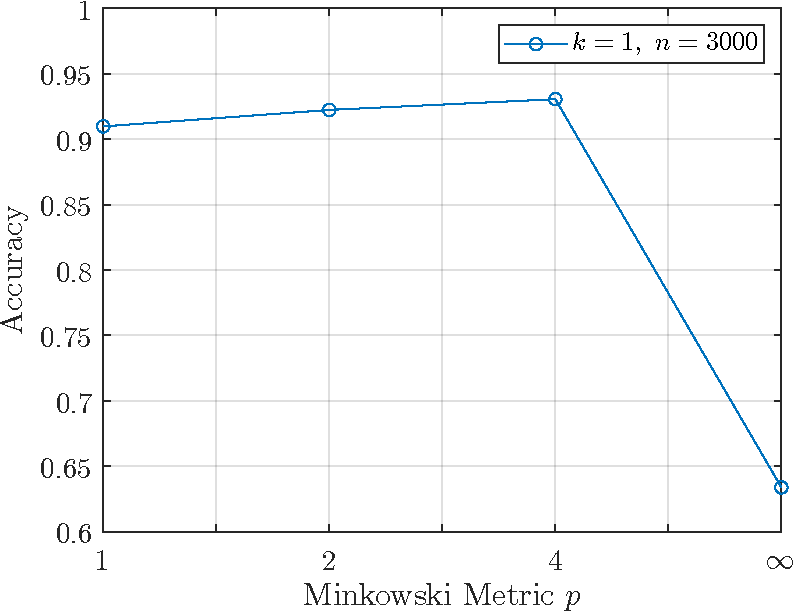
\includegraphics[width=8cm]{pAccuracy.pdf}
    \caption{正确率与 Minkowski 距离参数 $p$ 变化关系}
    \label{fig:pAccuracy}
  \end{minipage}
  \begin{minipage}[t]{0.48\textwidth}
    \centering
    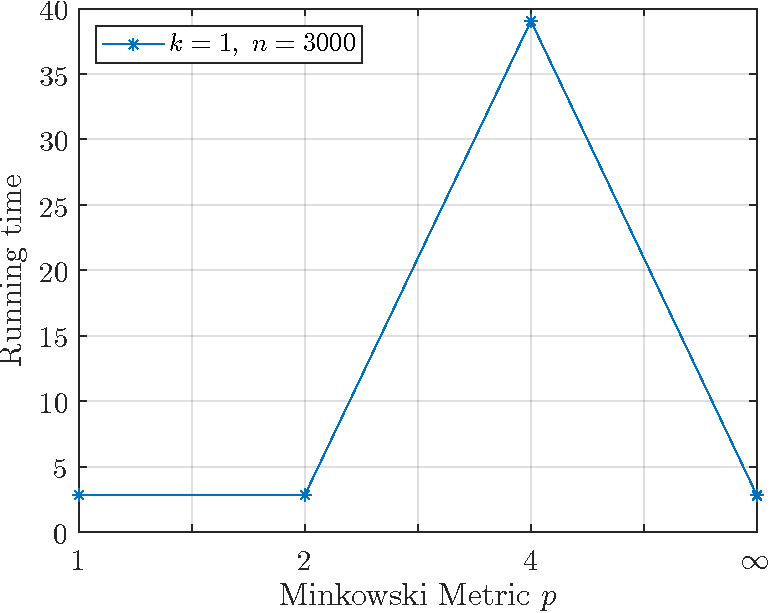
\includegraphics[width=8cm]{pTime.pdf}
    \caption{运行时间与 Minkowski 距离参数 $p$ 变化关系}
    \label{fig:pTime}
  \end{minipage}
\end{figure}

\section*{Literature Reading}
Please read a paper about metric learning \cite{metric_learning}.

\emph{Hint}: You do not have to submit anything for this reading section.

% Reference
\begin{thebibliography}{1}

\bibitem{pics}
File: Euclidean Voronoi diagram.svg. (2020, October 10). Wikimedia Commons, the free media repository. Retrieved 09:39, March 29, 2021 from 

\url{https://commons.wikimedia.org/wiki/File:Euclidean_Voronoi_diagram.svg}

\bibitem{ManhattanVoronoi}

File: Manhattan Voronoi Diagram.svg. (2020, September 17). Wikimedia Commons, the free media repository. Retrieved 08:26, June 19, 2021 from

\url{https://commons.wikimedia.org/wiki/File:Manhattan_Voronoi_Diagram.svg}

\bibitem{Holder_inequality}
J.M. Steele, The Cauchy-Schwarz Master Class, An Introduction to the Art of Mathematical Inequalities, MAA Problem Book Series,
Cambridge University Press, 2008.

\bibitem{mnist}
LeCun Y. The MNIST database of handwritten digits[J]. \url{http://yann.lecun.com/exdb/mnist/}, 1998.

\bibitem{metric_learning}
Xing E P, Ng A Y, Jordan M I, et al. Distance metric learning with application to clustering with side-information[C] // NIPS. 2002, 15(505–512): 12.

\end{thebibliography}

\end{document}
